In the literature, a multitude of meta-heuristic algorithms have emerged over
the years, exploring various ideas to guide the search
process~\cite{osman1996metaheuristics}. These encompass strategies that narrow
the search space to promising regions, enhance solutions in a greedy manner, or
utilize randomized and probabilistic techniques, some of which draw inspiration
from natural phenomena like collective behavior, natural selection, and physical
processes of materials.

However, the majority of state-of-the-art meta-heuristic algorithms can be
described by a couple of distinctive traits~\cite{blum2003metaheuristics} such as:

\begin{description}
  \item[\textbf{Search Strategy.}] This refers to the method used to construct a
    solution. It can be one of three main types: constructive (building step by
    step), local (making small improvements), or a composite approach that
    combines both strategies.

  \item[\textbf{Memoization.}] This concept involves maintaining a record or
    archive of previously explored solutions.~This record helps in identifying
    solutions that may be revisited or disregarded in subsequent stages of the
    optimization process.

  \item[\textbf{Population vs. Trajectory.}] This pertains to the number of
    solutions being evolved during the construction phase.~In~\emph{population
      methods}, multiple solutions are worked with at each iteration, while in
    ~\emph{trajectory methods}, only a single solution is dealt with at a time.
\end{description}

In this section, we will offer a brief overview of select state-of-the-art
\acrshort{meta-heuristic} algorithms, which encapsulate all the above properties
and will be utilized and implemented in the context of this work.

\subsection{Beam Search}
\label{subsec:beam-search}

\acrfull{beam-search}~\cite{ow1988filtered,outeiro2021application}

\begin{algorithm}
  \label{algorithm:beam-search}
  \caption{\acrlong{beam-search}}
  \begin{frame}{Problem}
  This problem entails the setup of scanning pipeline for books.

  \begin{itemize}
    \item There are libraries housing various books. Before any scanning can commence, each
          library needs to register for the scanning process. Once registered, each
          library is allowed to scan a certain number of books daily, until global deadline.
    \item Only one library can undergo the sign-up process at any given time.
    \item Each book, when scanned, contributes a specific score.
  \end{itemize}

\end{frame}

\begin{frame}{Example --- Book Scanning}
  \begin{figure}[h]
    \centering
    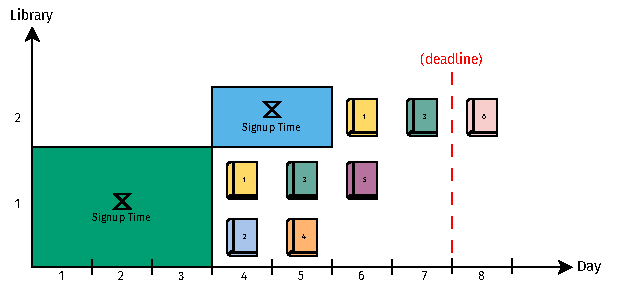
\includegraphics[width=0.8\textwidth,keepaspectratio]{../assets/bs/bs-example-slides.pdf}
    \caption{Book Scanning Example}
  \end{figure}

  \begin{table}[ht]
    \centering
    \begin{tabular}{ccccccc}
      \toprule
      \textbf{Book}  & 1 & 2 & 3 & 4 & 5 & 6 \\ \midrule
      \textbf{Score} & 3 & 1 & 5 & 4 & 7 & 1 \\
      \bottomrule
    \end{tabular}
    \caption{Book Scores}
  \end{table}
\end{frame}

\begin{frame}{Problem Formulation}
  \begin{equation*}
    \begin{aligned}
      \max\ f(x) =\  & \sum_{b = 1}^{\mathcal{B}}{s_{b} \cdot \min\left(\sum_{i = 1}^{\mathcal{I}}{x_{b, \phi_{i}^\mathcal{I}}} , 1\right)}                                                                     \\
      \text{s.t }    & \sum_{b = 1}^{\mathcal{B}}{x_{b, \phi_{i}^\mathcal{I}}} \leq r_{i} \cdot \left(\mathcal{D} - \sum_{k = 1}^{i}{t_{\phi_{k}^\mathcal{I}}} \right) \quad \forall i = 1, \ldots, \mathcal{I} \\
                     & \sum_{i = 1}^{\mathcal{I}}{t_{\phi_{i}^\mathcal{I}}} \leq \mathcal{D}                                                                                                                    \\
    \end{aligned}
  \end{equation*}
  Where,
  \begin{itemize}
    \item $\mathcal{B}$ is the number of books.
    \item $\mathcal{D}$ is the global deadline.
    \item $\mathcal{I}$ and $\phi^\mathcal{I}$ are the number and order of signed-up libraries.
    \item $t_{i}$ and $r_{i}$ are the sign-up time and book scanning rate of library $i$.
    \item $s_{b}$ is the score of book $b$.
    \item $x_{b,i}$ is binary variable indicating if a book, $b$, is assigned (1) or not (0) to library $i$.
  \end{itemize}
\end{frame}


\begin{frame}{Example --- Objective}
  \begin{figure}[h]
    \centering
    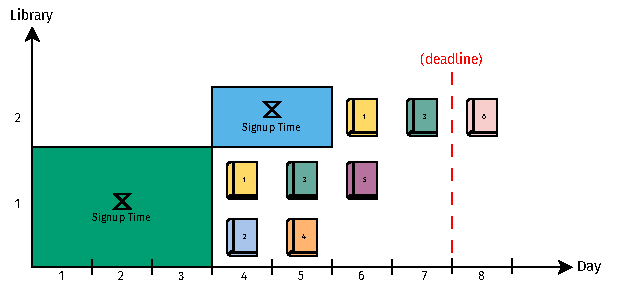
\includegraphics[width=0.8\textwidth,keepaspectratio]{../assets/bs/bs-example-slides.pdf}
  \end{figure}
  \begin{table}
    \begin{tabular}{cc}
      \begin{minipage}{0.5\textwidth}
        \begin{table}[ht]
          \centering
          \begin{tabular}{ccccccc}
            \toprule
            \textbf{Book}  & 1          & 2          & 3          & 4          & 5          & 6 \\ \midrule
            \textbf{Score} & \textbf{3} & \textbf{1} & \textbf{5} & \textbf{4} & \textbf{7} & 1 \\
            \bottomrule
          \end{tabular}
        \end{table}
      \end{minipage}
       &
      \begin{minipage}[b]{0.5\textwidth}
        \centering
        \begin{equation*}
          f(x) = 3 + 1 + 5 + 4 + 7 = 20
        \end{equation*}
      \end{minipage}
    \end{tabular}
    \caption{Book Scores \& Objective Value}
  \end{table}
\end{frame}

\begin{frame}{Modeling --- Problem, Solution and Component}
  The~\alert{problem} is characterized by the set of all libraries available, along with
  their sign-up times, book shipping rate, and list of books that can be shipped,
  the scores for all the books, and the deadline.

  A~\alert{solution} is characterized by a collection of assignments of books
  to libraries and the order in which libraries are scanned.

  A~\alert{component} is characterized by a tuple containing a book and a library or
  a tuple containing two libraries (denoting the sign-up order).
\end{frame}

\begin{frame}{Modeling --- Construction Rules}
  Two component enumeration strategies were considered:
  \begin{itemize}
    \item \textbf{Standard:} Enumerate all the books that can be scanned by all signed-up libraries
          as well as all libraries that can be signed-up until the deadline.
    \item \textbf{Sequential:} Enumerate only the books of the last signed-up library and all the libraries
          that can still be signed-up.
  \end{itemize}
\end{frame}

\begin{frame}{Modeling -- Upper Bound}
  The upper bounds were devised for this problem are as follows:
  \begin{enumerate}
    \item \textbf{Individual Library Knapsacks:} In this approach, we treat the
          number of books each library can scan before the deadline as an individual
          knapsack. The bound value for each library is calculated as the sum of
          scores from the best books that are yet to be scanned. The
          global upper bound is then determined by summing up the bound values for
          each library.

    \item \textbf{Combined Knapsack for All Libraries:} Consider a single
          knapsack representing the total number of books that can be scanned by
          all libraries combined until the deadline.
  \end{enumerate}
\end{frame}

\begin{frame}{Modeling -- Local Moves}
  The~\alert{local moves} considered for this problem are:

  \begin{enumerate}
    \item \textbf{Adding a book} to the set of books to be scanned by a given library.
    \item \textbf{Removing a book} from the set of books that were going to be scanned by a library.
    \item \textbf{Swapping books between libraries}.
    \item \textbf{Removing a book} from the list of books to be scanned by a library and
          \textbf{adding that book to another library}. If possible, ~\textbf{replace the removed book} in
          the first library~\textbf{with another one} that is available there.
  \end{enumerate}
\end{frame}

\begin{frame}{Modeling --- Two-Phase Approach}
  Use a meta-heuristic to choose an order for the libraries and solve the book assignment problem optimally.

  Notably, the assignment problem can be modeled as bipartite graph and solved with any
  \textbf{min cost max-flow} solver.

  \begin{figure}[h]
    \centering
    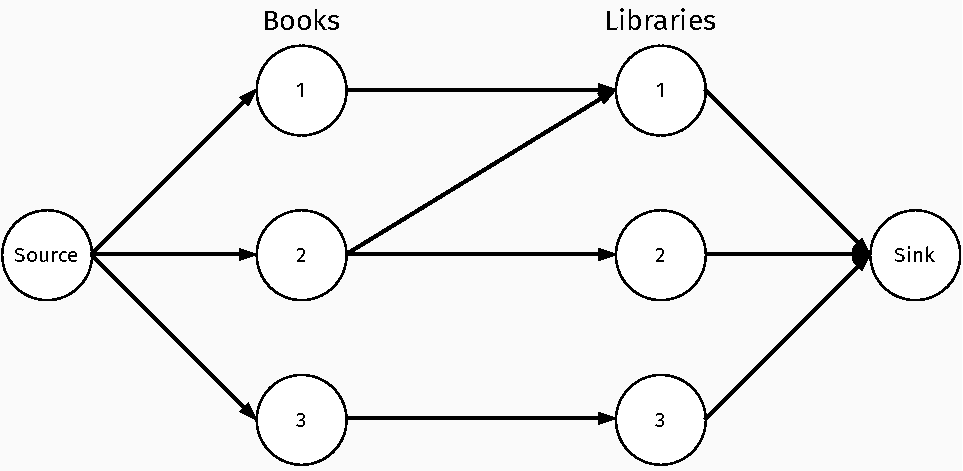
\includegraphics[width=0.8\textwidth,keepaspectratio]{../assets/bs/bs-graph-slides.pdf}
    \caption{Assignment Problem Modeled as a Bipartite Graph}
  \end{figure}
\end{frame}

\begin{frame}{Modeling --- Two-Phase Approach Local Moves}
  After the book assignment the solution can be further improved through
  the following~\alert{local moves}:
  \begin{enumerate}
    \item \textbf{Reverse the sign-up order} between two libraries.
    \item \textbf{Change the positions of two libraries} in the order adjusting the
          sign-up times of every library in between.
    \item \textbf{Select one library to remove and add another library} that is not
          currently considered in that position, if possible.
  \end{enumerate}
\end{frame}

\begin{frame}{Results}
  The best objective values for the five instance of this problem were obtained using the
  \textbf{two-phase} approach, as illustrated in the table below:

  \begin{table}[ht]
    \centering
    \begin{tabular}{@{\extracolsep{4pt}}lcc@{\extracolsep{4pt}}}
      \toprule
      Instance                           & Objective Value & Best Known Objective Value \\ \midrule
      \textquote{Read On}                & \num{5822900}   & \num{5822900}              \\
      \textquote{Incunabula}             & \num{5689822}   & \num{5690888}              \\
      \textquote{Tough Choices}          & \num{5028530}   & \num{5107113}              \\
      \textquote{So many books}          & \num{5208455}   & \num{5237345}              \\
      \textquote{Libraries of the world} & \num{5328034}   & \num{5348248}              \\
      \bottomrule
    \end{tabular}
    \caption{Book Scanning Best Results}
  \end{table}

  Remarkably, this objective value would have placed us in~\textbf{33rd}
  place~(out of 10716 teams) on the competition leaderboard.
\end{frame}
\end{algorithm}

\subsection{Iterated Greedy}
\label{subsec:iterated-greedy}

\acrfull{iterated-greedy}~\cite{stutzle2018iterated,outeiro2021application}

\begin{algorithm}
  \label{algorithm:iterated-greedy}
  \caption{\acrlong{iterated-greedy}}
  % Iterated Greedy (algorithm2e pseudocode)

\KwIn{Objective Function ($f$), Upper Bound Function($\Phi_{ub}$)}
\KwOut{Solution ($s^{*})$}

\SetKwFunction{Destruct}{\texttt{Destruct}}
\SetKwFunction{Construct}{\texttt{Construct}}
\SetKwFunction{LocalSearch}{\texttt{LocalSearch}}
\SetKwFunction{Accept}{\texttt{Accept}}

$s^{*}$ $\gets$ \Construct($\emptyset, \Phi_{ub}$)\;
\While{\texttt{stopping criteria not met}}{
  $s$ $\gets$ \Destruct{$s^{*}$}\;
  $s$ $\gets$ \Construct{$s, \Phi_{ub}$}\;
  \If{$s\ $ \texttt{is feasible} $\land$ $f(s) > f(s^{*})$}{
    $s^{*}$ $\gets$ $s'$\;
  }
}
\end{algorithm}

\subsection{Greedy Randomized Adaptive Search Procedure}
\label{subsec:grasp}

\acrfull{grasp}~\cite{resende2010greedya,outeiro2021application,blum2003metaheuristics}

% Greedy Randomized Adaptive Search Procedures
% (GRASP) are
% simple, single-state, stochastic meta-heuristics that iteratively build solutions by
% combining a greedy construction phase with a local search phase. The
% construction phase involves the selection of components from the ground set
% $\mathcal{G}$ based on their contribution to the objective function, using a
% greedy criterion, and subsequently incorporating them into a partial solution
% $s^{p}$. However, the constructed solution may not be feasible, requiring a
% repair process to improve its quality. The local search phase is then applied to
% the partial solution $s^{p}$ obtained during the construction phase, with the
% goal of further completing and improving the solution. The pseudo-code provided
% in Algorithm~\ref{algorithm:grasp} illustrates the functioning of a basic
% implementation of the GRASP algorithm.

\begin{algorithm}
  \label{algorithm:grasp}
  \caption{\acrlong{grasp}}
  % Greedy Randomized Adaptive Search Procedure (algorithm2e pseudocode)

\KwIn{Objective Function ($f$)}
\KwOut{Solution ($s^{*}$).}

\SetKwFunction{GreedyRandomizedConstruction}{\texttt{GreedyRandomizedConstruction}}
\SetKwFunction{LocalSearch}{\texttt{LocalSearch}}

$s^{*}$ $\gets$ $\emptyset$\;
\While{\texttt{stopping criteria not met}}{
  $s$ $\gets$ \GreedyRandomizedConstruction{}\;
  $s$ $\gets$ \LocalSearch{$s$}\;
  \If{$f(s)$ > $f(s^{*})$}{
    $s^{*}$ $\gets$ $s$\;
  }
}
\Return{$s^{*}$}
\end{algorithm}

\subsection{Ant Colony Optimization}
\label{subsec:aco}

\acrfull{aco}~\cite{dorigo2010anta,outeiro2021application,luke2013essentialsa,blum2003metaheuristics}

% Ant Colony Optimization (ACO is a population-based, stochastic,
% constructive meta-heuristic that is inspired by the foraging behavior of ants.
% 
% The algorithm simulates the movement of ``ants'' through the search space, where
% each ant constructs a solution by making a sequence of probabilistic choices
% based on the ``pheromone'' trail left by previous ants. Notably, the pheromones,
% associated with the components $c_{i}$ of the ground set $\mathcal{G}$, weigh
% the relevance of the integration of a specific component in a solution during
% the construction process.
% 
% One of the key features of ACO is the incorporation of a learning component
% through the use of a pheromone update rule that adapts the pheromone trail based
% on the quality of the solutions constructed by the ants, with the aim of guiding
% the ants towards better solutions over subsequent iterations. As such, the
% algorithm requires the tuning of several parameters such as the pheromone
% evaporation rate, the choice of the pheromone update rule, and the
% initialization of the pheromone trail.
% 
% In summary, the ACO meta-heuristic can be described as a process that comprises
% of a solution construction phase, in which solutions (referred to as ``ants'')
% are constructed, followed by an optional phase of exploiting these solutions
% through local search, and culminating in a pheromone update phase. This process
% is then repeated for multiple iterations, as can be observed in the pseudo-code
% provided in Algorithm ~\ref{algorithm:aco}.
% 
\begin{algorithm}
  \label{algorithm:aco}
  \caption{\acrlong{aco}}
  % Ant Colony Optimization (algorithm2e pseudocode)

\KwIn{Pheromone Update Rule ($\mathcal{R}$), Pheromone Values ($\vec{\tau}$), Evaporation Rate ($\alpha$)}
\KwOut{Solution ($s$)}

\SetKwFunction{AntBasedSolutionConstruction}{\texttt{AntBasedSolutionConstruction}}
\SetKwFunction{PheromoneUpdate}{\texttt{PheromoneUpdate}}
\SetKwFunction{LocalSearch}{\texttt{LocalSearch}}

$s \gets$ $s'$\;
$bobj$ $\gets$ $-\infty$\;
$\mathcal{S} \gets \{ \emptyset \}$\;

\If{ $s\ $ \texttt{is feasible}}{
  $bobj$ $\gets$ $f(s)$\;
}

\While{\texttt{not stopping criteria met}}{
  $\mathcal{S}$ $\gets$ \AntBasedSolutionConstruction{$\mathcal{S}$, $\vec{\tau}$}\;
  $\mathcal{S}$ $\gets$ \LocalSearch{$\mathcal{S}$} \Comment*[f]{Optional} \;
  $s'$ $\gets$ $\underset{s'\ \in\ \mathcal{S}}{\argmax}\ f(s')$ \Comment*[f]{Select best solution}\;
  \If{$f(s')$ > $bobj$}{
    $s \gets s'$\;
    $bobj$ $\gets$ $f(s')$\;
  }
  $\mathcal{S} \gets$ \PheromoneUpdate{$\mathcal{S}$, $\mathcal{R}$, $\vec{\tau}$, $\alpha$}\;
}
\Return{$s^{*}$}
\end{algorithm}

\subsection{Hill-Climbing}
\label{subsec:hill-climbing}

\acrfull{hill-climbing}~\cite{luke2013essentialsa,vieira2009uma} is a simple
stochastic, memory-less,~\acrshort{local-search} trajectory algorithm that works
by iteratively attempting to improve a starting solution through a sequence of
incremental changes,~\ie{}, by selecting the solution in the neighborhood that
yields the best increment with respect to the objective value. This process
terminates when the best solution possible is found or another stopping
criteria is met. Despite the simplicity of this method it is worth noting that,
due to the inherent greedy choice of the best at each step this approach is
susceptible to getting trapped in local optima. For illustration purposes the
pseudocode of simple version of an~\acrshort{hill-climbing} method is shown
in~\Cref{algorithm:hill-climbing}.

\begin{algorithm}
  % Hill Climbing (algorithm2e pseudocode)

\KwIn{Solution ($s$), Objective Function ($f$)}
\KwOut{Solution ($s$)}

\SetKwFunction{Perturb}{\texttt{Perturb}}

\While{ \texttt{stopping criteria not met} }{
  $s'$ $\gets$ \Perturb{$s$}\;
  \If{$f(s') > f(s)$}{
    $s$ $\gets$ $s'$\;
  }
}
\Return{ $s$ }
  \caption{\acrlong{hill-climbing}}
  \label{algorithm:hill-climbing}
\end{algorithm}

It's worth noting that the presented algorithm's effectiveness is rooted in the
efficiency of a random process, which strives to improve solution quality
through a sequence of perturbation attempts (\texttt{Perturb} function).
Nevertheless, there exist two noteworthy variations that more thoroughly explore
the solution's neighborhood and take steps in the direction of the most
substantial improvement. These are commonly known as~\acrfull{first-improvement}
and~\acrfull{best-improvement}. The latter is also known in the literature as
\textit{steepest ascent}~\acrshort{hill-climbing}~\cite{luke2013essentialsa}.

In a~\acrshort{first-improvement} approach, the first neighboring solution that
improves the current solution's quality is retained. Conversely, in a
\acrshort{best-improvement} scenario, the entire neighborhood of the current
solution is examined, and the best neighboring solution is selected for the
subsequent iteration.

\subsection{Iterated Local Search}
\label{subsec:iterated-local-search}

\acrfull{iterated-local-search}~\cite{lourenco2010iterateda,luke2013essentialsa,blum2003metaheuristics}

% The  is a single-state, stochastic, local search meta-heuristic
% that builds upon the ideas of Hill Climbing (HC) by incorporating repeated local
% searches starting from different solutions, allowing for exploration of the
% search space. In its simplest form, ILS can be implemented according to the
% pseudo-code shown in Algorithm~\ref{algorithm:iterated-local-search}. Variants
% of the ILS algorithm also exist, such as the memory-based, which store previously
% visited starting solutions to avoid re-exploration of the same regions of the
% search space.
% 
\begin{algorithm}
  \label{algorithm:iterated-local-search}
  \caption{\acrlong{iterated-local-search}}
  % Constructive Search Procedure (algorithm2e pseudocode)

\KwIn{Solution ($s$), Kick Strength ($k$), Objective Function ($f$)}
\KwOut{Solution ($s$).}

\SetKwFunction{Perturb}{\texttt{Perturb}}
\SetKwFunction{LocalSearch}{\texttt{LocalSearch}}

\While{\texttt{stopping criteria not met}}{
  $s'$ $\gets$ \LocalSearch{$s$}\;
  $s'$ $\gets$ \Perturb{$s', k$}\;
  \If{$f(s') > f(s$)}{
    $s$ $\gets$ $s'$\;
  }
}
\Return{$s$}
\end{algorithm}

\subsection{Simulated Annealing}
\label{subsec:simulated-annealing}

\acrfull{simulated-annealing}~\cite{kirkpatrick1983optimization,nikolaev2010simulateda,eglese1990simulated}

%is a single-state, stochastic, local
% search meta-heuristic that is inspired by the process of annealing in
% metallurgy.  The algorithm works by iteratively applying small perturbations to
% a candidate solution with the aim of improving it, and accepting new solutions
% based on their quality and a probability function that simulates the cooling
% process of a metal. The probability function is controlled by a temperature
% parameter, which gradually decreases over time, thus reducing the acceptance
% probability of worse solutions. This allows the algorithm to initially explore a
% wider range of solutions and escape local optima, ultimately improving the
% exploration of the search space. The details of the process can be found in the
% pseudo-code provided in Algorithm~\ref{algorithm:simmulated-annealing}.
% 
\begin{algorithm}
  \label{algorithm:simmulated-annealing}
  \caption{\acrlong{simulated-annealing}}
  % Simulated Annealing (algorithm2e pseudocode)

\KwIn{Solution ($s$), Initial Temperature ($t_{0}$), Cooling Rate ($\alpha$), Objective Function ($f$) }
\KwOut{Solution ($s$)}

\SetKwFunction{Random}{\texttt{Random}}
\SetKwFunction{Perturb}{\texttt{Perturb}}

$t \gets t_{0}$\;
\While{\texttt{stopping criteria not met}}{
  $s' \gets$ \Perturb{$s$}\;
  $\delta$ $\gets$ $f(s)$ - $f(s')$\;
  \If{$\delta < 0$ $\lor$ \Random{$0, 1$} $ < $ $e^{-\frac{\delta}{t}}$}{
    $s$ $\gets$ $s'$\;
  }
  $t$ $\gets$ $t \cdot \alpha$\;
}
\Return{$s$}
\end{algorithm}

\subsection{Tabu Search}
\label{subsec:tabu-search}

\acrfull{tabu-search}~\cite{glover1999tabu,gendreau2010tabua,luke2013essentialsa}

% Tabu Search (TS)~\cite{} is a single-state, stochastic, local search meta-heuristic
% that incorporates the use of memory to guide the search process. The algorithm
% iteratively explores the solution space by performing neighborhood searches for
% the best solutions, while maintaining a tabu list $\mathcal{T}$ of recently
% visited solutions that are temporarily forbidden from being revisited. The main
% idea behind this approach is that by avoiding previously visited solutions, the
% algorithm can escape local optima and explore new regions of the search space.
% The size and duration of the tabu list, as well as the rules for adding and
% removing solutions from the list, are user-specified parameters that need to be
% fine-tuned for each problem. The pseudo-code in
% Algorithm~\ref{algorithm:tabu-search} illustrates a simple version of this
% meta-heuristic.

\begin{algorithm}
  \label{algorithm:tabu-search}
  \caption{\acrlong{tabu-search}}
  % Tabu Search (algorithm2e pseudocode)

\KwIn{Solution ($s'$), Tabu Length ($l_{max}$), Objective Function ($f$)}
\KwOut{Solution ($s^{*}$)}

\SetKwFunction{Oldest}{\texttt{Oldest}}

$s^{*} \gets$ $s'$\;
$\mathcal{T}$ $\gets$ $\{ \emptyset \}$\;
\While{\texttt{stopping criteria not met}}{
  $s$ $\gets$ $\underset{s\ \in\ \mathcal{N}(s) \backslash \mathcal{T}}{\argmax}\ f(s)$ \Comment*[f]{Select best neighbor $s \notin \mathcal{T}$}\;
  \If{$f(s) > f(s^{*})$}{
    $s^{*}$ $\gets$ $s$\;
    $\mathcal{T} \gets \mathcal{T} \cup \{s\}$\;
  }
  \If{$\left\lvert \mathcal{T} \right\rvert$ $>$ $l_{\max}$} {
    $\mathcal{T}$ $\gets$ $\mathcal{T}\ \setminus $ \Oldest{$\mathcal{T}$}\;
  }
}
\Return{$s^{*}$}
\end{algorithm}

\subsection{Outline}
\label{subsec:Outline}